\section{Алгоритм расчета модели}

\tikzstyle{startstop} = [rectangle, rounded corners, minimum width=1.5cm, minimum height=1.5cm, text centered, draw=black, fill=red!20]
\tikzstyle{io} = [trapezium, trapezium left angle=70, trapezium right angle=110, minimum width=2cm, minimum height=1cm, text centered, text width=2cm, draw=black, fill=orange!20]
\tikzstyle{io2} = [trapezium, trapezium left angle=70, trapezium right angle=110, minimum width=3cm, minimum height=1cm, text centered, text width=3cm, draw=black, fill=orange!20]
\tikzstyle{process} = [rectangle, minimum width=2cm, minimum height=1cm, text centered, text width=2cm, draw=black, fill=blue!20]
\tikzstyle{process2} = [rectangle, minimum width=3cm, minimum height=1cm, text centered, text width=3cm, draw=black, fill=blue!20]
\tikzstyle{decision} = [diamond, minimum width=1cm, minimum height=1cm, text centered, draw=black, fill=green!20]
\tikzstyle{arrow} = [thick, ->, >=stealth]

\begin{frame}
\begin{center}
\frametitle{Алгоритм расчета модели}
\framesubtitle{Общая структура}
\begin{figure}
\begin{tikzpicture}[]
    \node (start) [startstop] {Старт};
    \node (read) [io2, right of=start, xshift=2.9cm]{Считать начальные условия и~параметры};
    \node (init) [process, right of=read, xshift=2.7cm] {t := $t_0$};
    \node (tloop) [decision, below of=init, yshift=-1.5cm] {t < $t_n$};
    \node (stop) [startstop, right of=tloop, xshift=1.8cm] {Стоп};
    \node (increment) [process, left of=tloop, xshift=-2.5cm] {t := t + $\Delta{t}$};
    \node (calc) [process, below of=tloop, right of=tloop, xshift=1cm, yshift=-2.0cm] {Применить граничные условия};
    \node (bound) [process, left of=calc, xshift=-1.9cm] {Вычислить $T(t)$, $P_w(t)$, $S_i(t)$};
    \node (net) [io, left of=bound, xshift=-2.1cm] {Передать данные по сети};
    \node (ioenable) [decision, left of=net, xshift=-2.0cm] {flush(t)};
    \node (save) [io, left of=increment, xshift=-2.5cm] {Сохранить в файл $T(t)$, $P_w(t)$, $S_i(t)$};

    \draw [arrow] (start) -- (read);
    \draw [arrow] (read) -- (init);
    \draw [arrow] (init) -- (tloop);
    \draw [arrow] (tloop) -- node[anchor=south] {Нет} (stop);
    \draw [arrow] (tloop) -- node[anchor=east] {Да} (calc);
    \draw [arrow] (calc) -- (bound);
    \draw [arrow] (save) -- (increment);
    \draw [arrow] (bound) -- (net);
    \draw [arrow] (net) -- (ioenable);
    \draw [arrow] (increment) -- (tloop);
    \draw [arrow] (ioenable) -- node[anchor=east] {Да} (save);
    \draw [arrow] (ioenable) -- node[anchor=west] {Нет} (increment);
\end{tikzpicture}
\end{figure}
\end{center}
\end{frame}


\begin{frame}
\begin{center}
\frametitle{Алгоритм расчета модели}
\framesubtitle{Вычисления на сетке}
\begin{figure}
\begin{tikzpicture}[]
    \node (start) [startstop] {Старт};
    \node (init) [process, right of=start, xshift=4.0cm] {x := $x_0$};
    \node (xloop) [decision, below of=init, yshift=-0.7cm] {x < $x_n$};
    \node (stop) [startstop, right of=xloop, xshift=4.0cm] {Стоп};
    \node (step) [process, left of=xloop, xshift=-3.0cm] {x := x + $\Delta{x}$};
    \node (active) [decision, below of=xloop, yshift=-1.2cm] {active(x)};
    \node (pressure) [process, right of=active, xshift=3.0cm] {Вычислить $P_n$, $P_g$ через $P_w$, $P_c$};
    \node (density) [process, below of=pressure, yshift=-1.0cm] {Вычислить $\mu_i$, $k_i$, $\rho_i$};
    \node (flux) [process2, left of=density, xshift=-3.0cm] {Вычислить $\rho_iS_i$ из уравнения неразрывности};
    \node (energy) [process2, left of=flux, xshift=-3.0cm] {Вычислить $E$ из уравнения сохранения энергии};
    \node (newton) [process2, below of=step, yshift=-1.0cm] {Найти с помощью метода Ньютона $T$, $P_w$, $S_i$};

    \draw [arrow] (start) -- (init);
    \draw [arrow] (init) -- (xloop);
    \draw [arrow] (xloop) -- node[anchor=west] {Да} (active);
    \draw [arrow] (active) -- node[anchor=north] {Да} (pressure);
    \draw [arrow] (active) -- node[anchor=west] {Нет} (step);
    \draw [arrow] (pressure) -- (density);
    \draw [arrow] (density) -- (flux);
    \draw [arrow] (flux) -- (energy);
    \draw [arrow] (energy) -- (newton);
    \draw [arrow] (xloop) -- node[anchor=south] {Нет} (stop);
    \draw [arrow] (newton) -- (step);
    \draw [arrow] (step) -- (xloop);
\end{tikzpicture}
\end{figure}
\end{center}
\end{frame}

\section{Параллельная реализация алгоритма}

\begin{frame}
\begin{center}
\frametitle{Параллельная реализация алгоритма}
\framesubtitle{Разбиение области по процессорам}
\begin{figure}
\begin{columns}[T]
\newcommand{\edje}{0.63}
\newcommand{\cl}{blue}
\begin{column}{.33\textwidth}
\begin{tikzpicture}[every node/.style={minimum size=1cm},on grid]
\begin{scope}[every node/.append style={yslant=-0.5},yslant=-0.5]
  \shade[right color=\cl!10, left color=\cl!50] (0,0) rectangle +(3*\edje,3*\edje);
  \draw[\cl] (0.0, 1.0*\edje) -- (3.0*\edje, 1.0*\edje);
  \draw[\cl] (0.0, 2.0*\edje) -- (3.0*\edje, 2.0*\edje);
  \draw[\cl] (0,0) rectangle (3*\edje,3*\edje);
\end{scope}
\begin{scope}[every node/.append style={yslant=0.5},yslant=0.5]
  \shade[right color=\cl!70,left color=\cl!10] (3*\edje,-3*\edje) rectangle +(3*\edje,3*\edje);
  \draw[\cl] (3.0*\edje, -2.0*\edje) -- (6.0*\edje, -2.0*\edje);
  \draw[\cl] (3.0*\edje, -1.0*\edje) -- (6.0*\edje, -1.0*\edje);
  \draw[\cl] (3*\edje,-3*\edje) rectangle (6*\edje,0);
\end{scope}
\begin{scope}[every node/.append style={
    yslant=0.5,xslant=-1},yslant=0.5,xslant=-1]
  \shade[bottom color=\cl!10, top color=\cl!80] (6*\edje,3*\edje) rectangle +(-3*\edje,-3*\edje);
  \draw[\cl] (3*\edje,0) rectangle (6*\edje,3*\edje);
\end{scope}
\end{tikzpicture}
\caption{Деление сетки в одном направлении}
\end{column}

\renewcommand{\cl}{purple}
\begin{column}{.33\textwidth}
\vspace{10mm}
\begin{tikzpicture}[every node/.style={minimum size=1cm},on grid]
\begin{scope}[every node/.append style={yslant=-0.5},yslant=-0.5]
  \shade[right color=\cl!10, left color=\cl!50] (0,0) rectangle +(3*\edje,3*\edje);
  \draw[\cl] (0.0, 1.0*\edje) -- (3.0*\edje, 1.0*\edje);
  \draw[\cl] (0.0, 2.0*\edje) -- (3.0*\edje, 2.0*\edje);
  \draw[\cl] (1.0*\edje, 0.0) -- (1.0*\edje, 3.0*\edje);
  \draw[\cl] (2.0*\edje, 0.0) -- (2.0*\edje, 3.0*\edje);
  \draw[\cl] (0,0) rectangle (3*\edje,3*\edje);
\end{scope}
\begin{scope}[every node/.append style={yslant=0.5},yslant=0.5]
  \shade[right color=\cl!70,left color=\cl!10] (3*\edje,-3*\edje) rectangle +(3*\edje,3*\edje);
  \draw[\cl] (3.0*\edje, -2.0*\edje) -- (6.0*\edje, -2.0*\edje);
  \draw[\cl] (3.0*\edje, -1.0*\edje) -- (6.0*\edje, -1.0*\edje);
  \draw[\cl] (3*\edje,-3*\edje) rectangle (6*\edje,0);
\end{scope}
\begin{scope}[every node/.append style={
    yslant=0.5,xslant=-1},yslant=0.5,xslant=-1]
  \shade[bottom color=\cl!10, top color=\cl!80] (6*\edje,3*\edje) rectangle +(-3*\edje,-3*\edje);
  \draw[\cl] (3.0*\edje, 1.0*\edje) -- (6.0*\edje, 1.0*\edje);
  \draw[\cl] (3.0*\edje, 2.0*\edje) -- (6.0*\edje, 2.0*\edje);
  \draw[\cl] (3*\edje,0) rectangle (6*\edje,3*\edje);
\end{scope}
\end{tikzpicture}
\caption{Деление сетки в двух направлениях}
\end{column}

\renewcommand{\cl}{red}
\begin{column}{.33\textwidth}
\begin{tikzpicture}[every node/.style={minimum size=1cm},on grid]
\begin{scope}[every node/.append style={yslant=-0.5},yslant=-0.5]
  \shade[right color=\cl!10, left color=\cl!50] (0,0) rectangle +(3*\edje,3*\edje);
  \draw[\cl] (0.0, 1.0*\edje) -- (3.0*\edje, 1.0*\edje);
  \draw[\cl] (0.0, 2.0*\edje) -- (3.0*\edje, 2.0*\edje);
  \draw[\cl] (1.0*\edje, 0.0) -- (1.0*\edje, 3.0*\edje);
  \draw[\cl] (2.0*\edje, 0.0) -- (2.0*\edje, 3.0*\edje);
  \draw[\cl] (0,0) rectangle (3*\edje,3*\edje);
\end{scope}
\begin{scope}[every node/.append style={yslant=0.5},yslant=0.5]
  \shade[right color=\cl!70,left color=\cl!10] (3*\edje,-3*\edje) rectangle +(3*\edje,3*\edje);
  \draw[\cl] (3.0*\edje, -2.0*\edje) -- (6.0*\edje, -2.0*\edje);
  \draw[\cl] (3.0*\edje, -1.0*\edje) -- (6.0*\edje, -1.0*\edje);
  \draw[\cl] (4.0*\edje, -3.0*\edje) -- (4.0*\edje, 0.0*\edje);
  \draw[\cl] (5.0*\edje, -3.0*\edje) -- (5.0*\edje, 0.0*\edje);
  \draw[\cl] (3*\edje,-3*\edje) rectangle (6*\edje,0);
\end{scope}
\begin{scope}[every node/.append style={
    yslant=0.5,xslant=-1},yslant=0.5,xslant=-1]
  \shade[bottom color=\cl!10, top color=\cl!80] (6*\edje,3*\edje) rectangle +(-3*\edje,-3*\edje);
  \draw[\cl] (3.0*\edje, 1.0*\edje) -- (6.0*\edje, 1.0*\edje);
  \draw[\cl] (3.0*\edje, 2.0*\edje) -- (6.0*\edje, 2.0*\edje);
  \draw[\cl] (4.0*\edje, 0.0*\edje) -- (4.0*\edje, 3.0*\edje);
  \draw[\cl] (5.0*\edje, 0.0*\edje) -- (5.0*\edje, 3.0*\edje);
  \draw[\cl] (3*\edje,0) rectangle (6*\edje,3*\edje);
\end{scope}
\end{tikzpicture}
\caption{Деление сетки в трех направлениях}
\end{column}
\end{columns}
\end{figure}
\end{center}
\end{frame}

\begin{frame}
\begin{center}
\frametitle{Параллельная реализация алгоритма}
\framesubtitle{Комплекс программ}
\begin{minipage}{0.5\textwidth}
\begin{itemize}
\item Параллельное решение 1D, 2D и 3D задач на произвольном числе CPU и GPU
\vspace{2mm}
\item Управление параметрами модели с помощью файла конфигурации
\vspace{2mm}
\item Технологии С/C++, MPI, CUDA, VTK (визуализация)
\vspace{2mm}
\item Кроссплатформенная реализация (Windows и Linux)
\vspace{2mm}
\item Сайт проекта \textcolor{blue}{https://github.com/alyupa/multiphase-flow-modeling}
\end{itemize}
\end{minipage}
\hfill
\begin{minipage}{0.45\textwidth}
  \begin{figure}
    \vspace{-2mm}
    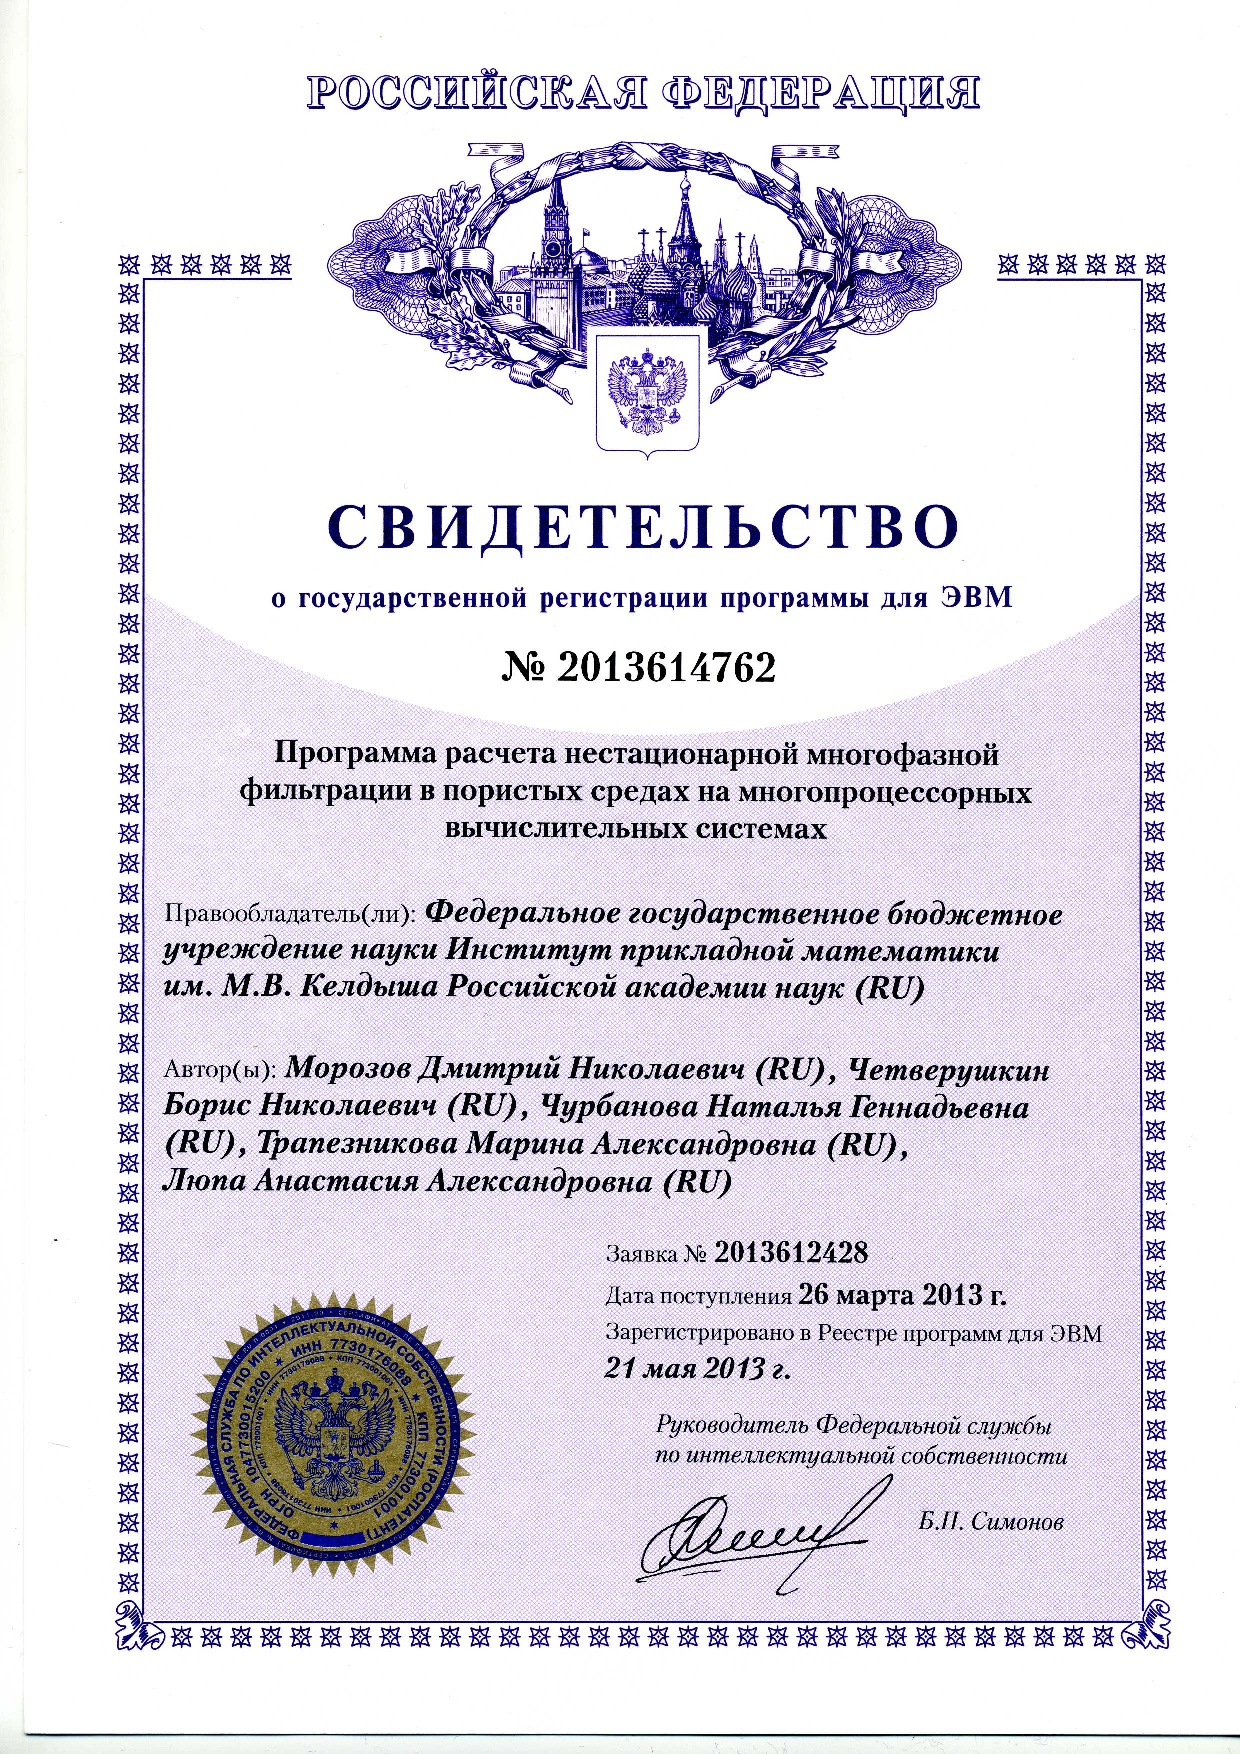
\includegraphics[height=0.9\textheight]{sert.pdf}
  \end{figure}
\end{minipage}
\end{center}
\end{frame}